% Created by tikzDevice version 0.12.6 on 2024-05-29 09:08:27
% !TEX encoding = UTF-8 Unicode
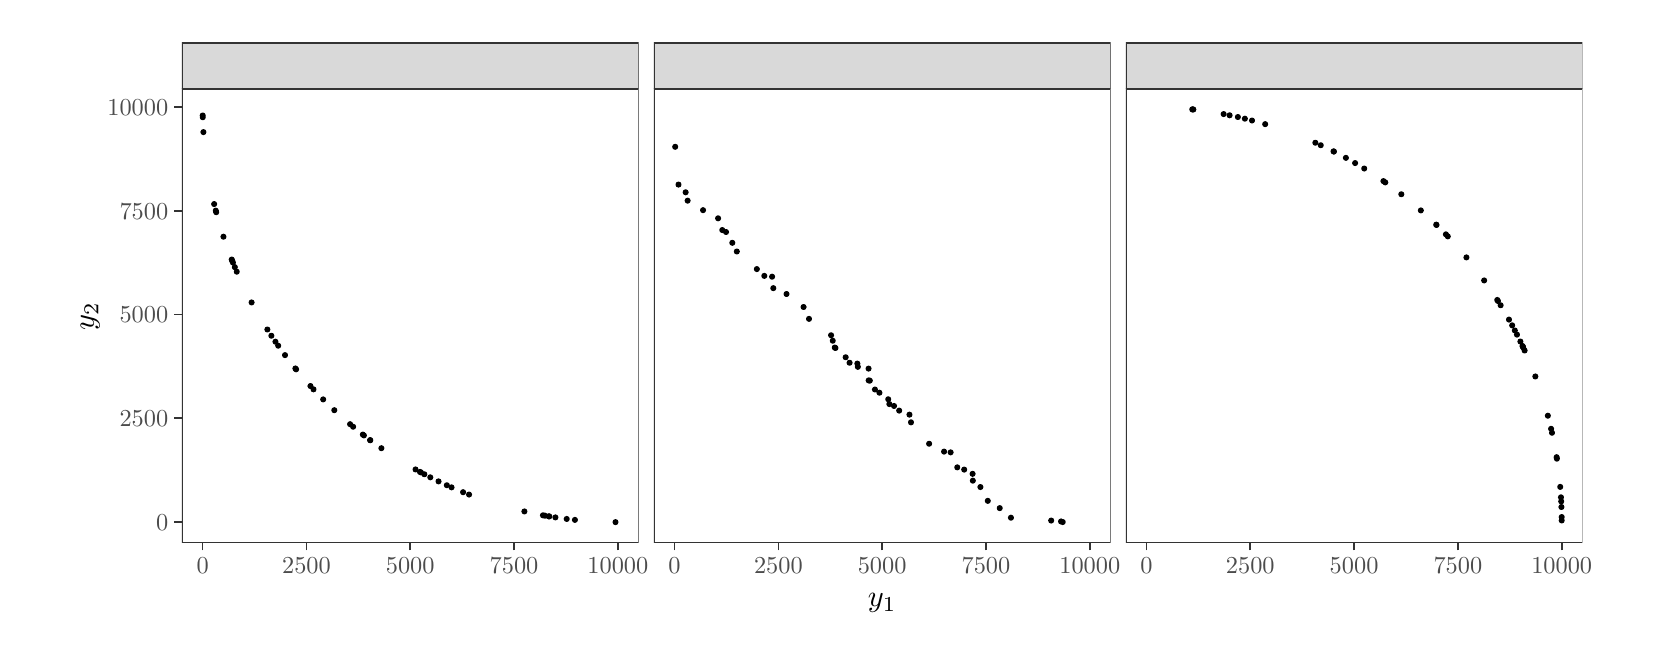
\begin{tikzpicture}[x=1pt,y=1pt]
\definecolor{fillColor}{RGB}{255,255,255}
\path[use as bounding box,fill=fillColor,fill opacity=0.00] (0,0) rectangle (578.16,216.81);
\begin{scope}
\path[clip] ( 10.84,  0.00) rectangle (567.32,216.81);
\definecolor{drawColor}{RGB}{255,255,255}
\definecolor{fillColor}{RGB}{255,255,255}

\path[draw=drawColor,line width= 0.6pt,line join=round,line cap=round,fill=fillColor] ( 10.84,  0.00) rectangle (567.32,216.81);
\end{scope}
\begin{scope}
\path[clip] ( 55.74, 30.69) rectangle (220.77,194.74);
\definecolor{fillColor}{RGB}{255,255,255}

\path[fill=fillColor] ( 55.74, 30.69) rectangle (220.77,194.74);
\definecolor{drawColor}{RGB}{0,0,0}
\definecolor{fillColor}{RGB}{0,0,0}

\path[draw=drawColor,line width= 0.4pt,line join=round,line cap=round,fill=fillColor] (141.77, 56.27) circle (  0.89);

\path[draw=drawColor,line width= 0.4pt,line join=round,line cap=round,fill=fillColor] (159.49, 48.11) circle (  0.89);

\path[draw=drawColor,line width= 0.4pt,line join=round,line cap=round,fill=fillColor] (194.78, 39.28) circle (  0.89);

\path[draw=drawColor,line width= 0.4pt,line join=round,line cap=round,fill=fillColor] ( 92.99, 98.48) circle (  0.89);

\path[draw=drawColor,line width= 0.4pt,line join=round,line cap=round,fill=fillColor] (123.79, 67.73) circle (  0.89);

\path[draw=drawColor,line width= 0.4pt,line join=round,line cap=round,fill=fillColor] (186.20, 40.60) circle (  0.89);

\path[draw=drawColor,line width= 0.4pt,line join=round,line cap=round,fill=fillColor] ( 86.61,107.74) circle (  0.89);

\path[draw=drawColor,line width= 0.4pt,line join=round,line cap=round,fill=fillColor] (116.50, 73.53) circle (  0.89);

\path[draw=drawColor,line width= 0.4pt,line join=round,line cap=round,fill=fillColor] ( 63.26,184.43) circle (  0.89);

\path[draw=drawColor,line width= 0.4pt,line join=round,line cap=round,fill=fillColor] (153.16, 50.70) circle (  0.89);

\path[draw=drawColor,line width= 0.4pt,line join=round,line cap=round,fill=fillColor] ( 90.53,101.89) circle (  0.89);

\path[draw=drawColor,line width= 0.4pt,line join=round,line cap=round,fill=fillColor] ( 68.12,150.13) circle (  0.89);

\path[draw=drawColor,line width= 0.4pt,line join=round,line cap=round,fill=fillColor] ( 74.17,131.93) circle (  0.89);

\path[draw=drawColor,line width= 0.4pt,line join=round,line cap=round,fill=fillColor] (145.48, 54.33) circle (  0.89);

\path[draw=drawColor,line width= 0.4pt,line join=round,line cap=round,fill=fillColor] (106.78, 82.48) circle (  0.89);

\path[draw=drawColor,line width= 0.4pt,line join=round,line cap=round,fill=fillColor] ( 73.87,132.66) circle (  0.89);

\path[draw=drawColor,line width= 0.4pt,line join=round,line cap=round,fill=fillColor] ( 75.55,128.63) circle (  0.89);

\path[draw=drawColor,line width= 0.4pt,line join=round,line cap=round,fill=fillColor] ( 63.25,185.08) circle (  0.89);

\path[draw=drawColor,line width= 0.4pt,line join=round,line cap=round,fill=fillColor] (121.50, 69.47) circle (  0.89);

\path[draw=drawColor,line width= 0.4pt,line join=round,line cap=round,fill=fillColor] ( 88.06,105.49) circle (  0.89);

\path[draw=drawColor,line width= 0.4pt,line join=round,line cap=round,fill=fillColor] (188.51, 40.20) circle (  0.89);

\path[draw=drawColor,line width= 0.4pt,line join=round,line cap=round,fill=fillColor] (143.34, 55.43) circle (  0.89);

\path[draw=drawColor,line width= 0.4pt,line join=round,line cap=round,fill=fillColor] (188.26, 40.24) circle (  0.89);

\path[draw=drawColor,line width= 0.4pt,line join=round,line cap=round,fill=fillColor] (148.46, 52.86) circle (  0.89);

\path[draw=drawColor,line width= 0.4pt,line join=round,line cap=round,fill=fillColor] (102.18, 87.32) circle (  0.89);

\path[draw=drawColor,line width= 0.4pt,line join=round,line cap=round,fill=fillColor] ( 96.99, 93.36) circle (  0.89);

\path[draw=drawColor,line width= 0.4pt,line join=round,line cap=round,fill=fillColor] (186.91, 40.47) circle (  0.89);

\path[draw=drawColor,line width= 0.4pt,line join=round,line cap=round,fill=fillColor] (197.74, 38.95) circle (  0.89);

\path[draw=drawColor,line width= 0.4pt,line join=round,line cap=round,fill=fillColor] ( 63.50,179.07) circle (  0.89);

\path[draw=drawColor,line width= 0.4pt,line join=round,line cap=round,fill=fillColor] (140.15, 57.17) circle (  0.89);

\path[draw=drawColor,line width= 0.4pt,line join=round,line cap=round,fill=fillColor] ( 96.74, 93.66) circle (  0.89);

\path[draw=drawColor,line width= 0.4pt,line join=round,line cap=round,fill=fillColor] (103.28, 86.12) circle (  0.89);

\path[draw=drawColor,line width= 0.4pt,line join=round,line cap=round,fill=fillColor] (179.49, 42.00) circle (  0.89);

\path[draw=drawColor,line width= 0.4pt,line join=round,line cap=round,fill=fillColor] ( 67.39,153.07) circle (  0.89);

\path[draw=drawColor,line width= 0.4pt,line join=round,line cap=round,fill=fillColor] (110.80, 78.58) circle (  0.89);

\path[draw=drawColor,line width= 0.4pt,line join=round,line cap=round,fill=fillColor] (127.81, 64.85) circle (  0.89);

\path[draw=drawColor,line width= 0.4pt,line join=round,line cap=round,fill=fillColor] ( 67.97,150.70) circle (  0.89);

\path[draw=drawColor,line width= 0.4pt,line join=round,line cap=round,fill=fillColor] (157.34, 48.95) circle (  0.89);

\path[draw=drawColor,line width= 0.4pt,line join=round,line cap=round,fill=fillColor] (190.70, 39.85) circle (  0.89);

\path[draw=drawColor,line width= 0.4pt,line join=round,line cap=round,fill=fillColor] ( 73.73,133.02) circle (  0.89);

\path[draw=drawColor,line width= 0.4pt,line join=round,line cap=round,fill=fillColor] ( 80.91,117.52) circle (  0.89);

\path[draw=drawColor,line width= 0.4pt,line join=round,line cap=round,fill=fillColor] ( 74.85,130.28) circle (  0.89);

\path[draw=drawColor,line width= 0.4pt,line join=round,line cap=round,fill=fillColor] (117.60, 72.60) circle (  0.89);

\path[draw=drawColor,line width= 0.4pt,line join=round,line cap=round,fill=fillColor] (212.41, 38.14) circle (  0.89);

\path[draw=drawColor,line width= 0.4pt,line join=round,line cap=round,fill=fillColor] ( 89.54,103.33) circle (  0.89);

\path[draw=drawColor,line width= 0.4pt,line join=round,line cap=round,fill=fillColor] (123.75, 67.76) circle (  0.89);

\path[draw=drawColor,line width= 0.4pt,line join=round,line cap=round,fill=fillColor] (121.11, 69.77) circle (  0.89);

\path[draw=drawColor,line width= 0.4pt,line join=round,line cap=round,fill=fillColor] (142.11, 56.09) circle (  0.89);

\path[draw=drawColor,line width= 0.4pt,line join=round,line cap=round,fill=fillColor] (151.46, 51.47) circle (  0.89);

\path[draw=drawColor,line width= 0.4pt,line join=round,line cap=round,fill=fillColor] ( 70.75,141.27) circle (  0.89);
\definecolor{drawColor}{gray}{0.20}

\path[draw=drawColor,line width= 0.6pt,line join=round,line cap=round] ( 55.74, 30.69) rectangle (220.77,194.74);
\end{scope}
\begin{scope}
\path[clip] (226.27, 30.69) rectangle (391.30,194.74);
\definecolor{fillColor}{RGB}{255,255,255}

\path[fill=fillColor] (226.27, 30.69) rectangle (391.30,194.74);
\definecolor{drawColor}{RGB}{0,0,0}
\definecolor{fillColor}{RGB}{0,0,0}

\path[draw=drawColor,line width= 0.4pt,line join=round,line cap=round,fill=fillColor] (244.04,150.86) circle (  0.89);

\path[draw=drawColor,line width= 0.4pt,line join=round,line cap=round,fill=fillColor] (268.99,126.82) circle (  0.89);

\path[draw=drawColor,line width= 0.4pt,line join=round,line cap=round,fill=fillColor] (319.18, 74.20) circle (  0.89);

\path[draw=drawColor,line width= 0.4pt,line join=round,line cap=round,fill=fillColor] (238.47,154.30) circle (  0.89);

\path[draw=drawColor,line width= 0.4pt,line join=round,line cap=round,fill=fillColor] (373.40, 38.38) circle (  0.89);

\path[draw=drawColor,line width= 0.4pt,line join=round,line cap=round,fill=fillColor] (310.96, 82.54) circle (  0.89);

\path[draw=drawColor,line width= 0.4pt,line join=round,line cap=round,fill=fillColor] (291.89,101.06) circle (  0.89);

\path[draw=drawColor,line width= 0.4pt,line join=round,line cap=round,fill=fillColor] (304.30, 89.27) circle (  0.89);

\path[draw=drawColor,line width= 0.4pt,line join=round,line cap=round,fill=fillColor] (233.98,173.76) circle (  0.89);

\path[draw=drawColor,line width= 0.4pt,line join=round,line cap=round,fill=fillColor] (296.99, 95.73) circle (  0.89);

\path[draw=drawColor,line width= 0.4pt,line join=round,line cap=round,fill=fillColor] (314.92, 78.43) circle (  0.89);

\path[draw=drawColor,line width= 0.4pt,line join=round,line cap=round,fill=fillColor] (333.50, 63.35) circle (  0.89);

\path[draw=drawColor,line width= 0.4pt,line join=round,line cap=round,fill=fillColor] (263.48,129.57) circle (  0.89);

\path[draw=drawColor,line width= 0.4pt,line join=round,line cap=round,fill=fillColor] (290.31,105.67) circle (  0.89);

\path[draw=drawColor,line width= 0.4pt,line join=round,line cap=round,fill=fillColor] (344.27, 50.82) circle (  0.89);

\path[draw=drawColor,line width= 0.4pt,line join=round,line cap=round,fill=fillColor] (269.43,122.68) circle (  0.89);

\path[draw=drawColor,line width= 0.4pt,line join=round,line cap=round,fill=fillColor] (346.93, 45.83) circle (  0.89);

\path[draw=drawColor,line width= 0.4pt,line join=round,line cap=round,fill=fillColor] (303.88, 89.34) circle (  0.89);

\path[draw=drawColor,line width= 0.4pt,line join=round,line cap=round,fill=fillColor] (280.36,115.87) circle (  0.89);

\path[draw=drawColor,line width= 0.4pt,line join=round,line cap=round,fill=fillColor] (291.63,101.23) circle (  0.89);

\path[draw=drawColor,line width= 0.4pt,line join=round,line cap=round,fill=fillColor] (369.84, 38.71) circle (  0.89);

\path[draw=drawColor,line width= 0.4pt,line join=round,line cap=round,fill=fillColor] (325.74, 66.46) circle (  0.89);

\path[draw=drawColor,line width= 0.4pt,line join=round,line cap=round,fill=fillColor] (374.01, 38.17) circle (  0.89);

\path[draw=drawColor,line width= 0.4pt,line join=round,line cap=round,fill=fillColor] (313.06, 80.11) circle (  0.89);

\path[draw=drawColor,line width= 0.4pt,line join=round,line cap=round,fill=fillColor] (256.24,135.93) circle (  0.89);

\path[draw=drawColor,line width= 0.4pt,line join=round,line cap=round,fill=fillColor] (295.58, 97.71) circle (  0.89);

\path[draw=drawColor,line width= 0.4pt,line join=round,line cap=round,fill=fillColor] (299.98, 94.25) circle (  0.89);

\path[draw=drawColor,line width= 0.4pt,line join=round,line cap=round,fill=fillColor] (252.35,142.97) circle (  0.89);

\path[draw=drawColor,line width= 0.4pt,line join=round,line cap=round,fill=fillColor] (282.33,111.59) circle (  0.89);

\path[draw=drawColor,line width= 0.4pt,line join=round,line cap=round,fill=fillColor] (338.41, 57.12) circle (  0.89);

\path[draw=drawColor,line width= 0.4pt,line join=round,line cap=round,fill=fillColor] (251.00,143.68) circle (  0.89);

\path[draw=drawColor,line width= 0.4pt,line join=round,line cap=round,fill=fillColor] (341.53, 53.12) circle (  0.89);

\path[draw=drawColor,line width= 0.4pt,line join=round,line cap=round,fill=fillColor] (235.17,160.11) circle (  0.89);

\path[draw=drawColor,line width= 0.4pt,line join=round,line cap=round,fill=fillColor] (335.90, 57.93) circle (  0.89);

\path[draw=drawColor,line width= 0.4pt,line join=round,line cap=round,fill=fillColor] (331.14, 63.62) circle (  0.89);

\path[draw=drawColor,line width= 0.4pt,line join=round,line cap=round,fill=fillColor] (237.75,157.32) circle (  0.89);

\path[draw=drawColor,line width= 0.4pt,line join=round,line cap=round,fill=fillColor] (303.85, 93.62) circle (  0.89);

\path[draw=drawColor,line width= 0.4pt,line join=round,line cap=round,fill=fillColor] (299.80, 95.42) circle (  0.89);

\path[draw=drawColor,line width= 0.4pt,line join=round,line cap=round,fill=fillColor] (266.18,127.12) circle (  0.89);

\path[draw=drawColor,line width= 0.4pt,line join=round,line cap=round,fill=fillColor] (249.48,147.92) circle (  0.89);

\path[draw=drawColor,line width= 0.4pt,line join=round,line cap=round,fill=fillColor] (341.44, 55.59) circle (  0.89);

\path[draw=drawColor,line width= 0.4pt,line join=round,line cap=round,fill=fillColor] (274.20,120.57) circle (  0.89);

\path[draw=drawColor,line width= 0.4pt,line join=round,line cap=round,fill=fillColor] (355.30, 39.73) circle (  0.89);

\path[draw=drawColor,line width= 0.4pt,line join=round,line cap=round,fill=fillColor] (318.63, 76.98) circle (  0.89);

\path[draw=drawColor,line width= 0.4pt,line join=round,line cap=round,fill=fillColor] (290.91,103.69) circle (  0.89);

\path[draw=drawColor,line width= 0.4pt,line join=round,line cap=round,fill=fillColor] (351.25, 43.20) circle (  0.89);

\path[draw=drawColor,line width= 0.4pt,line join=round,line cap=round,fill=fillColor] (311.37, 80.80) circle (  0.89);

\path[draw=drawColor,line width= 0.4pt,line join=round,line cap=round,fill=fillColor] (254.61,139.07) circle (  0.89);

\path[draw=drawColor,line width= 0.4pt,line join=round,line cap=round,fill=fillColor] (306.16, 86.06) circle (  0.89);

\path[draw=drawColor,line width= 0.4pt,line join=round,line cap=round,fill=fillColor] (307.78, 84.90) circle (  0.89);
\definecolor{drawColor}{gray}{0.20}

\path[draw=drawColor,line width= 0.6pt,line join=round,line cap=round] (226.27, 30.69) rectangle (391.30,194.74);
\end{scope}
\begin{scope}
\path[clip] (396.80, 30.69) rectangle (561.82,194.74);
\definecolor{fillColor}{RGB}{255,255,255}

\path[fill=fillColor] (396.80, 30.69) rectangle (561.82,194.74);
\definecolor{drawColor}{RGB}{0,0,0}
\definecolor{fillColor}{RGB}{0,0,0}

\path[draw=drawColor,line width= 0.4pt,line join=round,line cap=round,fill=fillColor] (536.42,109.24) circle (  0.89);

\path[draw=drawColor,line width= 0.4pt,line join=round,line cap=round,fill=fillColor] (540.40,101.27) circle (  0.89);

\path[draw=drawColor,line width= 0.4pt,line join=round,line cap=round,fill=fillColor] (550.48, 71.86) circle (  0.89);

\path[draw=drawColor,line width= 0.4pt,line join=round,line cap=round,fill=fillColor] (482.96,165.91) circle (  0.89);

\path[draw=drawColor,line width= 0.4pt,line join=round,line cap=round,fill=fillColor] (540.28,101.54) circle (  0.89);

\path[draw=drawColor,line width= 0.4pt,line join=round,line cap=round,fill=fillColor] (447.17,181.94) circle (  0.89);

\path[draw=drawColor,line width= 0.4pt,line join=round,line cap=round,fill=fillColor] (554.32, 38.74) circle (  0.89);

\path[draw=drawColor,line width= 0.4pt,line join=round,line cap=round,fill=fillColor] (439.83,183.92) circle (  0.89);

\path[draw=drawColor,line width= 0.4pt,line join=round,line cap=round,fill=fillColor] (526.29,125.47) circle (  0.89);

\path[draw=drawColor,line width= 0.4pt,line join=round,line cap=round,fill=fillColor] (540.14,101.80) circle (  0.89);

\path[draw=drawColor,line width= 0.4pt,line join=round,line cap=round,fill=fillColor] (552.48, 61.60) circle (  0.89);

\path[draw=drawColor,line width= 0.4pt,line join=round,line cap=round,fill=fillColor] (471.87,172.11) circle (  0.89);

\path[draw=drawColor,line width= 0.4pt,line join=round,line cap=round,fill=fillColor] (531.03,118.42) circle (  0.89);

\path[draw=drawColor,line width= 0.4pt,line join=round,line cap=round,fill=fillColor] (508.98,145.63) circle (  0.89);

\path[draw=drawColor,line width= 0.4pt,line join=round,line cap=round,fill=fillColor] (554.14, 45.63) circle (  0.89);

\path[draw=drawColor,line width= 0.4pt,line join=round,line cap=round,fill=fillColor] (554.31, 39.97) circle (  0.89);

\path[draw=drawColor,line width= 0.4pt,line join=round,line cap=round,fill=fillColor] (437.30,184.52) circle (  0.89);

\path[draw=drawColor,line width= 0.4pt,line join=round,line cap=round,fill=fillColor] (489.90,161.37) circle (  0.89);

\path[draw=drawColor,line width= 0.4pt,line join=round,line cap=round,fill=fillColor] (552.57, 61.07) circle (  0.89);

\path[draw=drawColor,line width= 0.4pt,line join=round,line cap=round,fill=fillColor] (535.27,111.32) circle (  0.89);

\path[draw=drawColor,line width= 0.4pt,line join=round,line cap=round,fill=fillColor] (531.27,118.05) circle (  0.89);

\path[draw=drawColor,line width= 0.4pt,line join=round,line cap=round,fill=fillColor] (476.33,169.77) circle (  0.89);

\path[draw=drawColor,line width= 0.4pt,line join=round,line cap=round,fill=fillColor] (421.21,187.24) circle (  0.89);

\path[draw=drawColor,line width= 0.4pt,line join=round,line cap=round,fill=fillColor] (532.24,116.50) circle (  0.89);

\path[draw=drawColor,line width= 0.4pt,line join=round,line cap=round,fill=fillColor] (553.78, 50.87) circle (  0.89);

\path[draw=drawColor,line width= 0.4pt,line join=round,line cap=round,fill=fillColor] (434.31,185.15) circle (  0.89);

\path[draw=drawColor,line width= 0.4pt,line join=round,line cap=round,fill=fillColor] (420.82,187.28) circle (  0.89);

\path[draw=drawColor,line width= 0.4pt,line join=round,line cap=round,fill=fillColor] (432.16,185.59) circle (  0.89);

\path[draw=drawColor,line width= 0.4pt,line join=round,line cap=round,fill=fillColor] (421.02,187.27) circle (  0.89);

\path[draw=drawColor,line width= 0.4pt,line join=round,line cap=round,fill=fillColor] (550.81, 70.43) circle (  0.89);

\path[draw=drawColor,line width= 0.4pt,line join=round,line cap=round,fill=fillColor] (513.15,141.40) circle (  0.89);

\path[draw=drawColor,line width= 0.4pt,line join=round,line cap=round,fill=fillColor] (442.41,183.26) circle (  0.89);

\path[draw=drawColor,line width= 0.4pt,line join=round,line cap=round,fill=fillColor] (512.47,142.12) circle (  0.89);

\path[draw=drawColor,line width= 0.4pt,line join=round,line cap=round,fill=fillColor] (540.91,100.15) circle (  0.89);

\path[draw=drawColor,line width= 0.4pt,line join=round,line cap=round,fill=fillColor] (509.08,145.52) circle (  0.89);

\path[draw=drawColor,line width= 0.4pt,line join=round,line cap=round,fill=fillColor] (465.30,175.23) circle (  0.89);

\path[draw=drawColor,line width= 0.4pt,line join=round,line cap=round,fill=fillColor] (549.31, 76.59) circle (  0.89);

\path[draw=drawColor,line width= 0.4pt,line join=round,line cap=round,fill=fillColor] (519.89,133.79) circle (  0.89);

\path[draw=drawColor,line width= 0.4pt,line join=round,line cap=round,fill=fillColor] (538.15,105.89) circle (  0.89);

\path[draw=drawColor,line width= 0.4pt,line join=round,line cap=round,fill=fillColor] (554.05, 47.10) circle (  0.89);

\path[draw=drawColor,line width= 0.4pt,line join=round,line cap=round,fill=fillColor] (467.25,174.33) circle (  0.89);

\path[draw=drawColor,line width= 0.4pt,line join=round,line cap=round,fill=fillColor] (554.22, 43.60) circle (  0.89);

\path[draw=drawColor,line width= 0.4pt,line join=round,line cap=round,fill=fillColor] (503.41,150.77) circle (  0.89);

\path[draw=drawColor,line width= 0.4pt,line join=round,line cap=round,fill=fillColor] (544.79, 90.77) circle (  0.89);

\path[draw=drawColor,line width= 0.4pt,line join=round,line cap=round,fill=fillColor] (472.02,172.04) circle (  0.89);

\path[draw=drawColor,line width= 0.4pt,line join=round,line cap=round,fill=fillColor] (496.36,156.61) circle (  0.89);

\path[draw=drawColor,line width= 0.4pt,line join=round,line cap=round,fill=fillColor] (537.38,107.39) circle (  0.89);

\path[draw=drawColor,line width= 0.4pt,line join=round,line cap=round,fill=fillColor] (539.39,103.40) circle (  0.89);

\path[draw=drawColor,line width= 0.4pt,line join=round,line cap=round,fill=fillColor] (479.67,167.88) circle (  0.89);

\path[draw=drawColor,line width= 0.4pt,line join=round,line cap=round,fill=fillColor] (490.57,160.90) circle (  0.89);
\definecolor{drawColor}{gray}{0.20}

\path[draw=drawColor,line width= 0.6pt,line join=round,line cap=round] (396.80, 30.69) rectangle (561.82,194.74);
\end{scope}
\begin{scope}
\path[clip] ( 55.74,194.74) rectangle (220.77,211.31);
\definecolor{drawColor}{gray}{0.20}
\definecolor{fillColor}{gray}{0.85}

\path[draw=drawColor,line width= 0.6pt,line join=round,line cap=round,fill=fillColor] ( 55.74,194.74) rectangle (220.77,211.31);
\definecolor{drawColor}{gray}{0.10}

\node[text=drawColor,anchor=base,inner sep=0pt, outer sep=0pt, scale=  0.88] at (138.26,199.99) {\mL};
\end{scope}
\begin{scope}
\path[clip] (226.27,194.74) rectangle (391.30,211.31);
\definecolor{drawColor}{gray}{0.20}
\definecolor{fillColor}{gray}{0.85}

\path[draw=drawColor,line width= 0.6pt,line join=round,line cap=round,fill=fillColor] (226.27,194.74) rectangle (391.30,211.31);
\definecolor{drawColor}{gray}{0.10}

\node[text=drawColor,anchor=base,inner sep=0pt, outer sep=0pt, scale=  0.88] at (308.78,199.99) {\mM};
\end{scope}
\begin{scope}
\path[clip] (396.80,194.74) rectangle (561.82,211.31);
\definecolor{drawColor}{gray}{0.20}
\definecolor{fillColor}{gray}{0.85}

\path[draw=drawColor,line width= 0.6pt,line join=round,line cap=round,fill=fillColor] (396.80,194.74) rectangle (561.82,211.31);
\definecolor{drawColor}{gray}{0.10}

\node[text=drawColor,anchor=base,inner sep=0pt, outer sep=0pt, scale=  0.88] at (479.31,199.99) {\mU};
\end{scope}
\begin{scope}
\path[clip] (  0.00,  0.00) rectangle (578.16,216.81);
\definecolor{drawColor}{gray}{0.20}

\path[draw=drawColor,line width= 0.6pt,line join=round] ( 63.22, 27.94) --
	( 63.22, 30.69);

\path[draw=drawColor,line width= 0.6pt,line join=round] (100.73, 27.94) --
	(100.73, 30.69);

\path[draw=drawColor,line width= 0.6pt,line join=round] (138.24, 27.94) --
	(138.24, 30.69);

\path[draw=drawColor,line width= 0.6pt,line join=round] (175.76, 27.94) --
	(175.76, 30.69);

\path[draw=drawColor,line width= 0.6pt,line join=round] (213.27, 27.94) --
	(213.27, 30.69);
\end{scope}
\begin{scope}
\path[clip] (  0.00,  0.00) rectangle (578.16,216.81);
\definecolor{drawColor}{gray}{0.30}

\node[text=drawColor,anchor=base,inner sep=0pt, outer sep=0pt, scale=  0.88] at ( 63.22, 19.68) {0};

\node[text=drawColor,anchor=base,inner sep=0pt, outer sep=0pt, scale=  0.88] at (100.73, 19.68) {2500};

\node[text=drawColor,anchor=base,inner sep=0pt, outer sep=0pt, scale=  0.88] at (138.24, 19.68) {5000};

\node[text=drawColor,anchor=base,inner sep=0pt, outer sep=0pt, scale=  0.88] at (175.76, 19.68) {7500};

\node[text=drawColor,anchor=base,inner sep=0pt, outer sep=0pt, scale=  0.88] at (213.27, 19.68) {10000};
\end{scope}
\begin{scope}
\path[clip] (  0.00,  0.00) rectangle (578.16,216.81);
\definecolor{drawColor}{gray}{0.20}

\path[draw=drawColor,line width= 0.6pt,line join=round] (233.74, 27.94) --
	(233.74, 30.69);

\path[draw=drawColor,line width= 0.6pt,line join=round] (271.26, 27.94) --
	(271.26, 30.69);

\path[draw=drawColor,line width= 0.6pt,line join=round] (308.77, 27.94) --
	(308.77, 30.69);

\path[draw=drawColor,line width= 0.6pt,line join=round] (346.28, 27.94) --
	(346.28, 30.69);

\path[draw=drawColor,line width= 0.6pt,line join=round] (383.80, 27.94) --
	(383.80, 30.69);
\end{scope}
\begin{scope}
\path[clip] (  0.00,  0.00) rectangle (578.16,216.81);
\definecolor{drawColor}{gray}{0.30}

\node[text=drawColor,anchor=base,inner sep=0pt, outer sep=0pt, scale=  0.88] at (233.74, 19.68) {0};

\node[text=drawColor,anchor=base,inner sep=0pt, outer sep=0pt, scale=  0.88] at (271.26, 19.68) {2500};

\node[text=drawColor,anchor=base,inner sep=0pt, outer sep=0pt, scale=  0.88] at (308.77, 19.68) {5000};

\node[text=drawColor,anchor=base,inner sep=0pt, outer sep=0pt, scale=  0.88] at (346.28, 19.68) {7500};

\node[text=drawColor,anchor=base,inner sep=0pt, outer sep=0pt, scale=  0.88] at (383.80, 19.68) {10000};
\end{scope}
\begin{scope}
\path[clip] (  0.00,  0.00) rectangle (578.16,216.81);
\definecolor{drawColor}{gray}{0.20}

\path[draw=drawColor,line width= 0.6pt,line join=round] (404.27, 27.94) --
	(404.27, 30.69);

\path[draw=drawColor,line width= 0.6pt,line join=round] (441.78, 27.94) --
	(441.78, 30.69);

\path[draw=drawColor,line width= 0.6pt,line join=round] (479.30, 27.94) --
	(479.30, 30.69);

\path[draw=drawColor,line width= 0.6pt,line join=round] (516.81, 27.94) --
	(516.81, 30.69);

\path[draw=drawColor,line width= 0.6pt,line join=round] (554.32, 27.94) --
	(554.32, 30.69);
\end{scope}
\begin{scope}
\path[clip] (  0.00,  0.00) rectangle (578.16,216.81);
\definecolor{drawColor}{gray}{0.30}

\node[text=drawColor,anchor=base,inner sep=0pt, outer sep=0pt, scale=  0.88] at (404.27, 19.68) {0};

\node[text=drawColor,anchor=base,inner sep=0pt, outer sep=0pt, scale=  0.88] at (441.78, 19.68) {2500};

\node[text=drawColor,anchor=base,inner sep=0pt, outer sep=0pt, scale=  0.88] at (479.30, 19.68) {5000};

\node[text=drawColor,anchor=base,inner sep=0pt, outer sep=0pt, scale=  0.88] at (516.81, 19.68) {7500};

\node[text=drawColor,anchor=base,inner sep=0pt, outer sep=0pt, scale=  0.88] at (554.32, 19.68) {10000};
\end{scope}
\begin{scope}
\path[clip] (  0.00,  0.00) rectangle (578.16,216.81);
\definecolor{drawColor}{gray}{0.30}

\node[text=drawColor,anchor=base east,inner sep=0pt, outer sep=0pt, scale=  0.88] at ( 50.79, 35.11) {0};

\node[text=drawColor,anchor=base east,inner sep=0pt, outer sep=0pt, scale=  0.88] at ( 50.79, 72.63) {2500};

\node[text=drawColor,anchor=base east,inner sep=0pt, outer sep=0pt, scale=  0.88] at ( 50.79,110.14) {5000};

\node[text=drawColor,anchor=base east,inner sep=0pt, outer sep=0pt, scale=  0.88] at ( 50.79,147.65) {7500};

\node[text=drawColor,anchor=base east,inner sep=0pt, outer sep=0pt, scale=  0.88] at ( 50.79,185.17) {10000};
\end{scope}
\begin{scope}
\path[clip] (  0.00,  0.00) rectangle (578.16,216.81);
\definecolor{drawColor}{gray}{0.20}

\path[draw=drawColor,line width= 0.6pt,line join=round] ( 52.99, 38.14) --
	( 55.74, 38.14);

\path[draw=drawColor,line width= 0.6pt,line join=round] ( 52.99, 75.66) --
	( 55.74, 75.66);

\path[draw=drawColor,line width= 0.6pt,line join=round] ( 52.99,113.17) --
	( 55.74,113.17);

\path[draw=drawColor,line width= 0.6pt,line join=round] ( 52.99,150.68) --
	( 55.74,150.68);

\path[draw=drawColor,line width= 0.6pt,line join=round] ( 52.99,188.20) --
	( 55.74,188.20);
\end{scope}
\begin{scope}
\path[clip] (  0.00,  0.00) rectangle (578.16,216.81);
\definecolor{drawColor}{RGB}{0,0,0}

\node[text=drawColor,anchor=base,inner sep=0pt, outer sep=0pt, scale=  1.10] at (308.78,  7.64) {$y_1$};
\end{scope}
\begin{scope}
\path[clip] (  0.00,  0.00) rectangle (578.16,216.81);
\definecolor{drawColor}{RGB}{0,0,0}

\node[text=drawColor,rotate= 90.00,anchor=base,inner sep=0pt, outer sep=0pt, scale=  1.10] at ( 23.91,112.71) {$y_2$};
\end{scope}
\end{tikzpicture}
